
%% bare_conf.tex
%% V1.4b
%% 2015/08/26
%% by Michael Shell
%% See:
%% http://www.michaelshell.org/
%% for current contact information.
%%
%% This is a skeleton file demonstrating the use of IEEEtran.cls
%% (requires IEEEtran.cls version 1.8b or later) with an IEEE
%% conference paper.
%%
%% Support sites:
%% http://www.michaelshell.org/tex/ieeetran/
%% http://www.ctan.org/pkg/ieeetran
%% and
%% http://www.ieee.org/

%%*************************************************************************
%% Legal Notice:
%% This code is offered as-is without any warranty either expressed or
%% implied; without even the implied warranty of MERCHANTABILITY or
%% FITNESS FOR A PARTICULAR PURPOSE! 
%% User assumes all risk.
%% In no event shall the IEEE or any contributor to this code be liable for
%% any damages or losses, including, but not limited to, incidental,
%% consequential, or any other damages, resulting from the use or misuse
%% of any information contained here.
%%
%% All comments are the opinions of their respective authors and are not
%% necessarily endorsed by the IEEE.
%%
%% This work is distributed under the LaTeX Project Public License (LPPL)
%% ( http://www.latex-project.org/ ) version 1.3, and may be freely used,
%% distributed and modified. A copy of the LPPL, version 1.3, is included
%% in the base LaTeX documentation of all distributions of LaTeX released
%% 2003/12/01 or later.
%% Retain all contribution notices and credits.
%% ** Modified files should be clearly indicated as such, including  **
%% ** renaming them and changing author support contact information. **
%%*************************************************************************


% *** Authors should verify (and, if needed, correct) their LaTeX system  ***
% *** with the testflow diagnostic prior to trusting their LaTeX platform ***
% *** with production work. The IEEE's font choices and paper sizes can   ***
% *** trigger bugs that do not appear when using other class files.       ***                          ***
% The testflow support page is at:
% http://www.michaelshell.org/tex/testflow/



\documentclass[conference]{IEEEtran}
% Some Computer Society conferences also require the compsoc mode option,
% but others use the standard conference format.
%
% If IEEEtran.cls has not been installed into the LaTeX system files,
% manually specify the path to it like:
% \documentclass[conference]{../sty/IEEEtran}





% Some very useful LaTeX packages include:
% (uncomment the ones you want to load)


% *** MISC UTILITY PACKAGES ***
%
%\usepackage{ifpdf}
% Heiko Oberdiek's ifpdf.sty is very useful if you need conditional
% compilation based on whether the output is pdf or dvi.
% usage:
% \ifpdf
%   % pdf code
% \else
%   % dvi code
% \fi
% The latest version of ifpdf.sty can be obtained from:
% http://www.ctan.org/pkg/ifpdf
% Also, note that IEEEtran.cls V1.7 and later provides a builtin
% \ifCLASSINFOpdf conditional that works the same way.
% When switching from latex to pdflatex and vice-versa, the compiler may
% have to be run twice to clear warning/error messages.






% *** CITATION PACKAGES ***
%
%\usepackage{cite}
% cite.sty was written by Donald Arseneau
% V1.6 and later of IEEEtran pre-defines the format of the cite.sty package
% \cite{} output to follow that of the IEEE. Loading the cite package will
% result in citation numbers being automatically sorted and properly
% "compressed/ranged". e.g., [1], [9], [2], [7], [5], [6] without using
% cite.sty will become [1], [2], [5]--[7], [9] using cite.sty. cite.sty's
% \cite will automatically add leading space, if needed. Use cite.sty's
% noadjust option (cite.sty V3.8 and later) if you want to turn this off
% such as if a citation ever needs to be enclosed in parenthesis.
% cite.sty is already installed on most LaTeX systems. Be sure and use
% version 5.0 (2009-03-20) and later if using hyperref.sty.
% The latest version can be obtained at:
% http://www.ctan.org/pkg/cite
% The documentation is contained in the cite.sty file itself.






% *** GRAPHICS RELATED PACKAGES ***
%
\usepackage[pdftex]{graphicx}
  % declare the path(s) where your graphic files are
% \graphicspath{./figs/}
  % and their extensions so you won't have to specify these with
  % every instance of \includegraphics
\DeclareGraphicsExtensions{.pdf,.jpeg,.png}

\ifCLASSINFOpdf
  % \usepackage[pdftex]{graphicx}
  % declare the path(s) where your graphic files are
  % \graphicspath{{../pdf/}{../jpeg/}}
  % and their extensions so you won't have to specify these with
  % every instance of \includegraphics
  % \DeclareGraphicsExtensions{.pdf,.jpeg,.png}
\else
  % or other class option (dvipsone, dvipdf, if not using dvips). graphicx
  % will default to the driver specified in the system graphics.cfg if no
  % driver is specified.
  % \usepackage[dvips]{graphicx}
  % declare the path(s) where your graphic files are
  % \graphicspath{{../eps/}}
  % and their extensions so you won't have to specify these with
  % every instance of \includegraphics
  % \DeclareGraphicsExtensions{.eps}
\fi
% graphicx was written by David Carlisle and Sebastian Rahtz. It is
% required if you want graphics, photos, etc. graphicx.sty is already
% installed on most LaTeX systems. The latest version and documentation
% can be obtained at: 
% http://www.ctan.org/pkg/graphicx
% Another good source of documentation is "Using Imported Graphics in
% LaTeX2e" by Keith Reckdahl which can be found at:
% http://www.ctan.org/pkg/epslatex
%
% latex, and pdflatex in dvi mode, support graphics in encapsulated
% postscript (.eps) format. pdflatex in pdf mode supports graphics
% in .pdf, .jpeg, .png and .mps (metapost) formats. Users should ensure
% that all non-photo figures use a vector format (.eps, .pdf, .mps) and
% not a bitmapped formats (.jpeg, .png). The IEEE frowns on bitmapped formats
% which can result in "jaggedy"/blurry rendering of lines and letters as
% well as large increases in file sizes.
%
% You can find documentation about the pdfTeX application at:
% http://www.tug.org/applications/pdftex





% *** MATH PACKAGES ***
%
%\usepackage{amsmath}
% A popular package from the American Mathematical Society that provides
% many useful and powerful commands for dealing with mathematics.
%
% Note that the amsmath package sets \interdisplaylinepenalty to 10000
% thus preventing page breaks from occurring within multiline equations. Use:
%\interdisplaylinepenalty=2500
% after loading amsmath to restore such page breaks as IEEEtran.cls normally
% does. amsmath.sty is already installed on most LaTeX systems. The latest
% version and documentation can be obtained at:
% http://www.ctan.org/pkg/amsmath





% *** SPECIALIZED LIST PACKAGES ***
%
%\usepackage{algorithmic}
% algorithmic.sty was written by Peter Williams and Rogerio Brito.
% This package provides an algorithmic environment fo describing algorithms.
% You can use the algorithmic environment in-text or within a figure
% environment to provide for a floating algorithm. Do NOT use the algorithm
% floating environment provided by algorithm.sty (by the same authors) or
% algorithm2e.sty (by Christophe Fiorio) as the IEEE does not use dedicated
% algorithm float types and packages that provide these will not provide
% correct IEEE style captions. The latest version and documentation of
% algorithmic.sty can be obtained at:
% http://www.ctan.org/pkg/algorithms
% Also of interest may be the (relatively newer and more customizable)
% algorithmicx.sty package by Szasz Janos:
% http://www.ctan.org/pkg/algorithmicx




% *** ALIGNMENT PACKAGES ***
%
%\usepackage{array}
% Frank Mittelbach's and David Carlisle's array.sty patches and improves
% the standard LaTeX2e array and tabular environments to provide better
% appearance and additional user controls. As the default LaTeX2e table
% generation code is lacking to the point of almost being broken with
% respect to the quality of the end results, all users are strongly
% advised to use an enhanced (at the very least that provided by array.sty)
% set of table tools. array.sty is already installed on most systems. The
% latest version and documentation can be obtained at:
% http://www.ctan.org/pkg/array


% IEEEtran contains the IEEEeqnarray family of commands that can be used to
% generate multiline equations as well as matrices, tables, etc., of high
% quality.




% *** SUBFIGURE PACKAGES ***
%\ifCLASSOPTIONcompsoc
%  \usepackage[caption=false,font=normalsize,labelfont=sf,textfont=sf]{subfig}
%\else
%  \usepackage[caption=false,font=footnotesize]{subfig}
%\fi
% subfig.sty, written by Steven Douglas Cochran, is the modern replacement
% for subfigure.sty, the latter of which is no longer maintained and is
% incompatible with some LaTeX packages including fixltx2e. However,
% subfig.sty requires and automatically loads Axel Sommerfeldt's caption.sty
% which will override IEEEtran.cls' handling of captions and this will result
% in non-IEEE style figure/table captions. To prevent this problem, be sure
% and invoke subfig.sty's "caption=false" package option (available since
% subfig.sty version 1.3, 2005/06/28) as this is will preserve IEEEtran.cls
% handling of captions.
% Note that the Computer Society format requires a larger sans serif font
% than the serif footnote size font used in traditional IEEE formatting
% and thus the need to invoke different subfig.sty package options depending
% on whether compsoc mode has been enabled.
%
% The latest version and documentation of subfig.sty can be obtained at:
% http://www.ctan.org/pkg/subfig




% *** FLOAT PACKAGES ***
%
%\usepackage{fixltx2e}
% fixltx2e, the successor to the earlier fix2col.sty, was written by
% Frank Mittelbach and David Carlisle. This package corrects a few problems
% in the LaTeX2e kernel, the most notable of which is that in current
% LaTeX2e releases, the ordering of single and double column floats is not
% guaranteed to be preserved. Thus, an unpatched LaTeX2e can allow a
% single column figure to be placed prior to an earlier double column
% figure.
% Be aware that LaTeX2e kernels dated 2015 and later have fixltx2e.sty's
% corrections already built into the system in which case a warning will
% be issued if an attempt is made to load fixltx2e.sty as it is no longer
% needed.
% The latest version and documentation can be found at:
% http://www.ctan.org/pkg/fixltx2e


%\usepackage{stfloats}
% stfloats.sty was written by Sigitas Tolusis. This package gives LaTeX2e
% the ability to do double column floats at the bottom of the page as well
% as the top. (e.g., "\begin{figure*}[!b]" is not normally possible in
% LaTeX2e). It also provides a command:
%\fnbelowfloat
% to enable the placement of footnotes below bottom floats (the standard
% LaTeX2e kernel puts them above bottom floats). This is an invasive package
% which rewrites many portions of the LaTeX2e float routines. It may not work
% with other packages that modify the LaTeX2e float routines. The latest
% version and documentation can be obtained at:
% http://www.ctan.org/pkg/stfloats
% Do not use the stfloats baselinefloat ability as the IEEE does not allow
% \baselineskip to stretch. Authors submitting work to the IEEE should note
% that the IEEE rarely uses double column equations and that authors should try
% to avoid such use. Do not be tempted to use the cuted.sty or midfloat.sty
% packages (also by Sigitas Tolusis) as the IEEE does not format its papers in
% such ways.
% Do not attempt to use stfloats with fixltx2e as they are incompatible.
% Instead, use Morten Hogholm'a dblfloatfix which combines the features
% of both fixltx2e and stfloats:
%
% \usepackage{dblfloatfix}
% The latest version can be found at:
% http://www.ctan.org/pkg/dblfloatfix




% *** PDF, URL AND HYPERLINK PACKAGES ***
%
\usepackage{url}
% url.sty was written by Donald Arseneau. It provides better support for
% handling and breaking URLs. url.sty is already installed on most LaTeX
% systems. The latest version and documentation can be obtained at:
% http://www.ctan.org/pkg/url
% Basically, \url{my_url_here}.




% *** Do not adjust lengths that control margins, column widths, etc. ***
% *** Do not use packages that alter fonts (such as pslatex).         ***
% There should be no need to do such things with IEEEtran.cls V1.6 and later.
% (Unless specifically asked to do so by the journal or conference you plan
% to submit to, of course. )


% correct bad hyphenation here
\hyphenation{op-tical net-works semi-conduc-tor}


\begin{document}
%
% paper title
% Titles are generally capitalized except for words such as a, an, and, as,
% at, but, by, for, in, nor, of, on, or, the, to and up, which are usually
% not capitalized unless they are the first or last word of the title.
% Linebreaks \\ can be used within to get better formatting as desired.
% Do not put math or special symbols in the title.
\title{Mining Pre-Exposure Prophylaxis Trends \\ in Social Media}


% author names and affiliations
% use a multiple column layout for up to three different
% affiliations
\author{\IEEEauthorblockN{Patrick Breen}
\IEEEauthorblockA{Institute of Bioinformatics\\
University of Georgia\\
Athens, Georgia\\
Email: pbreen@uga.edu}
\and
\IEEEauthorblockN{Jane Kelly}
\IEEEauthorblockA{ Georgia Department of \\Public Health\\
Atlanta, Georgia\\
Email: Jane.Kelly@dph.ga.gov}
\and
\IEEEauthorblockN{Timothy Heckman}
\IEEEauthorblockA{College of Public Health\\
University of Georgia\\
Athens, Georgia\\
Email: heckman@uga.edu}
\and
\IEEEauthorblockN{Shannon Quinn}
\IEEEauthorblockA{Department of \\Computer Science\\
University of Georgia\\
Athens, Georgia\\
Email: squinn@cs.uga.edu}
}
%\IEEEauthorblockN{Homer Simpson}
%\IEEEauthorblockA{Twentieth Century Fox\\
%Springfield, USA\\
%Email: homer@thesimpsons.com}
%\and
%\IEEEauthorblockN{James Kirk\\ and Montgomery Scott}
%\IEEEauthorblockA{Starfleet Academy\\
%San Francisco, California 96678--2391\\
%Telephone: (800) 555--1212\\
%Fax: (888) 555--1212}}

% conference papers do not typically use \thanks and this command
% is locked out in conference mode. If really needed, such as for
% the acknowledgment of grants, issue a \IEEEoverridecommandlockouts
% after \documentclass

% for over three affiliations, or if they all won't fit within the width
% of the page, use this alternative format:
% 
%\author{\IEEEauthorblockN{Michael Shell\IEEEauthorrefmark{1},
%Homer Simpson\IEEEauthorrefmark{2},
%James Kirk\IEEEauthorrefmark{3}, 
%Montgomery Scott\IEEEauthorrefmark{3} and
%Eldon Tyrell\IEEEauthorrefmark{4}}
%\IEEEauthorblockA{\IEEEauthorrefmark{1}School of Electrical and Computer Engineering\\
%Georgia Institute of Technology,
%Atlanta, Georgia 30332--0250\\ Email: see http://www.michaelshell.org/contact.html}
%\IEEEauthorblockA{\IEEEauthorrefmark{2}Twentieth Century Fox, Springfield, USA\\
%Email: homer@thesimpsons.com}
%\IEEEauthorblockA{\IEEEauthorrefmark{3}Starfleet Academy, San Francisco, California 96678-2391\\
%Telephone: (800) 555--1212, Fax: (888) 555--1212}
%\IEEEauthorblockA{\IEEEauthorrefmark{4}Tyrell Inc., 123 Replicant Street, Los Angeles, California 90210--4321}}




% use for special paper notices
%\IEEEspecialpapernotice{(Invited Paper)}




% make the title area
\maketitle

% As a general rule, do not put math, special symbols or citations
% in the abstract
\begin{abstract}

Pre-Exposure Prophylaxis (PrEP) is a ground-breaking biomedical approach to curbing the transmission of Human Immunodeficiency Virus (HIV). Truvada, the most common form of PrEP, is a combination of tenofovir and emtricitabine and is a once-daily oral mediation taken by HIV-seronegative persons at elevated risk for HIV infection. When taken reliably every day, PrEP can reduce one's risk for HIV infection by as much as 99\%. While highly efficacious, PrEP is expensive, somewhat stigmatized, and many health care providers remain uninformed about its benefits. Data mining of social media can monitor the spread of HIV in the United States, but no study has investigated PrEP use and sentiment via social media. This paper describes a data mining and machine learning strategy using natural language processing (NLP) that monitors Twitter social media data to identify PrEP discussion trends. Results showed that we can identify PrEP and HIV discussion dynamics over time, and assign PrEP-related tweets positive or negative sentiment. Results can enable public health professionals to monitor PrEP discussion trends and identify strategies to improve HIV prevention via PrEP.

\end{abstract}

% no keywords




% For peer review papers, you can put extra information on the cover
% page as needed:
% \ifCLASSOPTIONpeerreview
% \begin{center} \bfseries EDICS Category: 3-BBND \end{center}
% \fi
%
% For peerreview papers, this IEEEtran command inserts a page break and
% creates the second title. It will be ignored for other modes.
\IEEEpeerreviewmaketitle



\section{Introduction}

Pre-exposure prophylaxis (PrEP), a treatment for the prevention of Human Immunodeficiency Virus (HIV), is marketed under the trade name Truvada. Truvada, a combination of tenofovir and emtricitabine, was approved by the Food and Drug Administration (FDA) in 2012 to prevent the transmission of HIV to seronegative persons at elevated risk for HIV infection. Several randomized clinical trials showed that PrEP was safe and could reduce one's risk for HIV infection by up to 99\% if taken reliably~\cite{grant2010preexposure,thigpen2012antiretroviral}. Despite its minimal side effects and high level of risk protection, PrEP suffers from uncertain health insurance compensation, the risk of producing drug resistant strains, and uninformed health providers and patients~\cite{liu2014early}. Truvada must be taken once a day for maximum protection. Consistent adherence to PrEP is difficult for some individuals, leading to lower protection rates~\cite{van2012unraveling}. While public health officials can disseminate information about and monitor the efficacy of PrEP at the clinic-level, scaled-up data mining on social media data may provide more complete information on facilitators and barriers to PrEP use at the national level.

Twitter, a popular microblogging service, is the social media platform we use in this study. ``Tweets'' from Twitter consist of short 140 character text messages that may also contain hashtag annotations. Twitter has been used as a source of data for large scale opinion mining in public health monitoring contexts, to predict the spread of influenza~\cite{aramaki2011twitter}, predict postpartum depression~\cite{de2013predicting}, and examine tobacco use~\cite{myslin2013using}. Recently it has also been used for the study of HIV~\cite{young2014methods,young2013online}. These studies of HIV have focused on county-level HIV prevalence prediction, and general HIV discussion monitoring, but they have not focused on PrEP-related discussion. Furthermore, existing HIV social media analyses have not taken full advantage of natural language processing (NLP) techniques to discover semantic information in unstructured text~\cite{young2015big}.

In this paper we respond to the acknowledged need to harness large scale data in the battle against HIV~\cite{young2015big}. We make extensive use of NLP techniques to extract PrEP-related semantic information from a Twitter corpus dataset. We identify critical PrEP related terms, users, hashtags and tweets. We identify PrEP discussion trends over time, and identify other topics that co-occur with who tweet about PrEP. Finally we train a sentiment classifier that automatically identifies PrEP-related tweets with positive and negative sentiment. Together these results, and these approaches, can be used by public health officials to identify trends in the national PrEP discussion and respond to public health issues as they arise.

\section{Methods and Data}

One recently developed tool for NLP, called word2vec, is a connectionist method that embeds words as word-vectors in a semantic space that captures substitution-similarity~\cite{mikolov2013efficient}. There are several forms of word2vec, though the most popular version, Skip-gram Negative Sampling (SGNS), has been shown to perform well at producing word-vectors that capture important word relationships. This includes most notably word analogies. 

Word2vec is also used as a preprocessing step for additional analyses that start from pre-trained word-vectors. Doc2vec~\cite{le2014distributed} is one such method that uses pre-trained word-vectors to produce a document-vector for each document-level attribute. In the case of a tweet-corpus, document identifiers might include tweet ID, hashtags, and the user who created the tweet. Each of these document-level identifiers is embedded in a similarity space, allowing one to identify similar tweets, hastags, and users.

Latent Dirichlet Allocation~\cite{blei2003latent} (LDA) is used to identify a small set of latent topics present in an unstructured corpus. LDA is a graphical model that generates documents from a set of latent topics. A topic is a probability distribution over words that captures a set of related words. LDA models are often inferred in practice using Bayesian inference either via collapsed Gibbs sampling or variational Bayesian methods. Inspection of the resulting topics allows one to identify relevant terms and the context in which they occur in the corpus. 

Dynamic Topic Modeling~\cite{blei2006dynamic} (DTM) is an extension of LDA that produces a series of topic models over time. Briefly, the documents in the corpus are divided into several corpora that are successive in time. LDA is performed on each corpus to extract a topic distribution. The posterior topic distribution from time $t_n$ is used as the prior for time $t_{n+1}$. This lets the DTM model determine a topic model for each time point that is dependent both on the set of tweets from that time point, and on the previous time point's topic distribution.

We collected 624,569 tweets containing at least one of the following words `HIV', `AIDS', `truvada', `prophylaxis', `imtesting', or `PrEP' from Twitter's streaming API. The tweets were restricted to English language, and the collection dates spanned from the 47th week of 2015 to the 14th week of 2016. The tweets were cleaned of exotic characters (non-punctuation, non-alphanumeric characters). Before performing topic analysis, we excluded words that were mentioned fewer than 10 times, or more than 0.3 times the number of documents. We also performed Term Frequency Inverse Document Frequency (TF-IDF) normalization.

We excluded tweets that did not originate in contiguous United States time zones. A subset of 14,204 tweets (about 2\%) had geolocation coordinates available. We found that these tweets were largely concentrated on US and Canadian metro areas (Fig.~\ref{fig:map}). The tweets did not seem to be over represented in any geographical region of the US.

\section{Results}

We sought to determine trends in HIV and PrEP discourse on Twitter to inform and coordinate public health efforts aiming to promote PrEP adoption and adherence for at-risk individuals. 

% figure 1
\begin{figure}
\centering
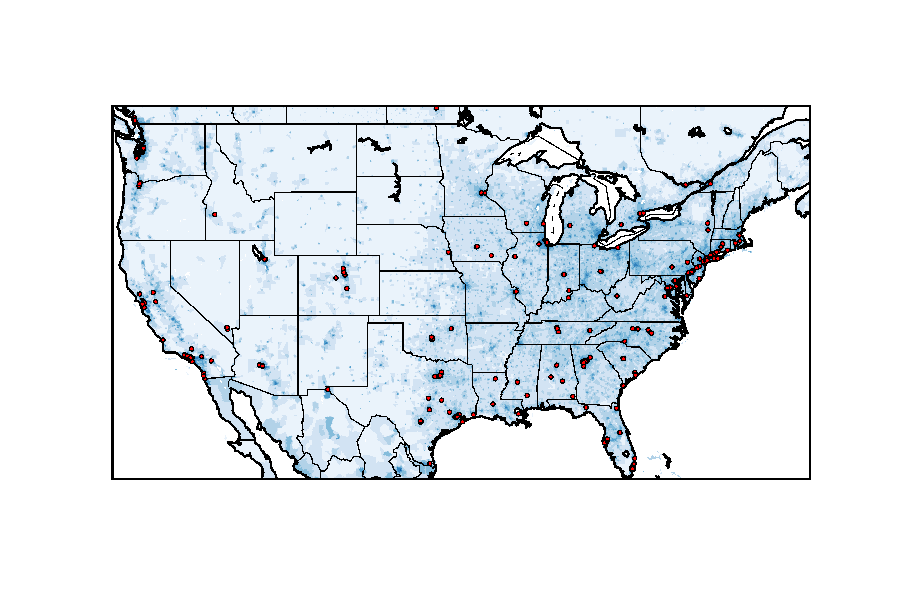
\includegraphics[scale=0.5]{figs/Fig1}
\caption{Plot of geolocated tweets.}
\label{fig:map}
\end{figure}

\subsection{Word and Document Similarity}

The first analysis that we performed sought to identify certain keywords, hashtags, tweets and users, that were discussed in HIV and PrEP related contexts. Word2vec and the related method, doc2vec, are unsupervised machine learning methods that have performed well at embedding natural language in a semantic vector space. In our analysis, word2vec allows us to determine semantically similar words to a query word, while doc2vec allows us to determine similar tweets, users and hashtags to a query hashtag.

We trained a word2vec model on the filtered dataset of 624,569 tweets, and queried for the top 10 word-vectors related to the term PrEP (Table~\ref{tbl:w2v}). We found several HIV/AIDS related events, WorldAIDSDay, HLM2016AIDS, ICASA2015, as well as the PrEP drug Truvada, and the term HIV. In addition, we found the acronym ART which refers to Anti-Retroviral Therapy. DoingIt, and OneConversation, are ongoing efforts led by the Center for Disease Control (CDC) to spread awareness and reduce the spread of HIV. NBHAAD is an organization that is committed to increasing awareness for HIV within the Black community. Nancy Reagan, who died in early 2016, was mentioned in conjunction with her efforts to combat HIV in the 1980's. Together these results show us a high-level view of the important components of the national PrEP conversation on Twitter over the collection period.

% table 1 - w2v PrEP
\begin{table}
\centering
\caption{Cosine similarity to word-vector ``PrEP''}
\begin{tabular}{|l|c|} \hline
Related word & Cosine similarity to PrEP\\ \hline
truvada & 0.796666\\ \hline
DoingIt & 0.738141\\ \hline
WorldAIDSDay & 0.720910\\ \hline
NancyReagan & 0.717667\\ \hline
NBHAAD & 0.705061\\ \hline
ART & 0.704300\\ \hline
HLM2016AIDS & 0.698698\\ \hline
ICASA2015 & 0.693117\\ \hline
HIV & 0.692860\\ \hline
OneConversation & 0.688427\\ \hline
\hline\end{tabular}
\label{tbl:w2v}
\end{table}

Doc2vec allows us to identify the top users, tweets, and hashtags associated with \#prep. Note that on Twitter, hashtags are not case-sensitive. Querying for the top 10 document-level entities associated with \#prep, we again see several PrEP and HIV related hashtags including \#hiv, \#hivprevention, \#truvada, and \#whereisprep. We also see an LGBT-related hashtag, \#lgbtmedia16, which indicates a distinct awareness of PrEP in the Gay community. This may reflect the elevated levels of HIV transmission in men who have sex with men~\cite{centers2014hiv}. Together the doc2vec results show that we can monitor and identify PrEP-related hashtags and tweets.

Interestingly, we also found 3 tweets and 1 user in the top 10 doc2vec results for \#prep (Table~\ref{tbl:d2v}). Tweet 702179860983189504 has content spreading HIV prevention awareness: ``\#StoneColdVideoTODAY if You see this 13 symptoms. Do HIV Test Immediately. Must Read''. Conversely tweet 708519265540907010 has content that calls into doubt the usefulness of PrEP: ``Checkout why PrEP is hurting the cause \& \#JoinTheConversation \#LGBTQIA''.

We investigated the blog article linked to tweet 708519265540907010~\cite{prephurtingcause}. The article, authored by Steven Banning, an HIV positive individual, expresses concerns about how new HIV treatments, like PrEP are being adopted by the HIV community. Steven notes that treatments for HIV positive individuals, and treatments to prevent HIV such as PrEP, have made HIV a much more treatable disease than it was in the 1980's. These medical advances may have led in part to some unintended medical and social consequences. Steven notes that the rise of drug-resistant HIV strains has increased, in part due to HIV patients not adhering to to consistent treatment plans. He also points out the recent social trend of ``bug chasers,'' individuals who are actively seeking to acquire and spread HIV strains. Steven Banning suggests that the widespread availability of effective HIV medications, may have desensitized a healthy sense of fear of the disease in some individuals.

User 711275699529764864 appears to be a Twitter spam bot with no obvious connection to PrEP. Unfortunately, bots are commonly used on Twitter for advertising and marketing purposes, and sometimes hinder pertinent information retrieval. Thus while we observe some noise, our results demonstrate a method to quickly identify and monitor the most viral tweets related to PrEP. As the discussion changes, public health professionals can use this information to quickly identify the most relevant viral sentiment in the online PrEP conversation.

% table 2 - d2v PrEP
\begin{table}
\centering
\caption{Cosine similarity to document-vector ``\#PrEP''}
\begin{tabular}{|l|c|} \hline
Related hashtag/tweet & Cosine similarity to \#PrEP\\ \hline
\#lgbtmedia16 & 0.739128\\ \hline
\#hiv & 	0.727602 \\ \hline
\#whereisprep & 0.707165 \\ \hline
\#truvada & 0.696113 \\ \hline
\#hivprevention & 0.636068 \\ \hline
tweet-702179860983189504 & 0.630055\\ \hline
user-711275699529764864 & 0.629254\\ \hline
tweet-708519265540907010 & 0.628778 \\ \hline
tweet-712032637024653313 & 0.628646 \\ \hline
\#harrogatehour & 0.628547 \\ \hline
\hline\end{tabular}
\label{tbl:d2v}
\end{table}

Finally we wanted to visualize the relative similarities of several PrEP-related keywords in a low dimensional space. We took keywords that we had identified in our PrEP related queries, along with other HIV-prevention related terms, and visualized their word-vectors in 2 dimensions using t-distributed Stochastic Neighborhood Embedding(tSNE)~\cite{van2008visualizing} (Fig.~\ref{fig:tsne}).

We identified several trends. Notably the pharmaceutical based HIV therapies all cluster together (ART, PrEP, truvada) and the AIDS awareness events cluster together (WorldAIDSDay, NBHAAD, ICASA2015). Words that are related to HIV discussion, but also used in other contexts (undetectable, testing, awareness) are further away from the HIV/AIDS word-clusters. These results demonstrate another mechanism for researchers to visualize and identify relevant trends in PrEP-related keywords.

% figure 2
\begin{figure*}
\centering
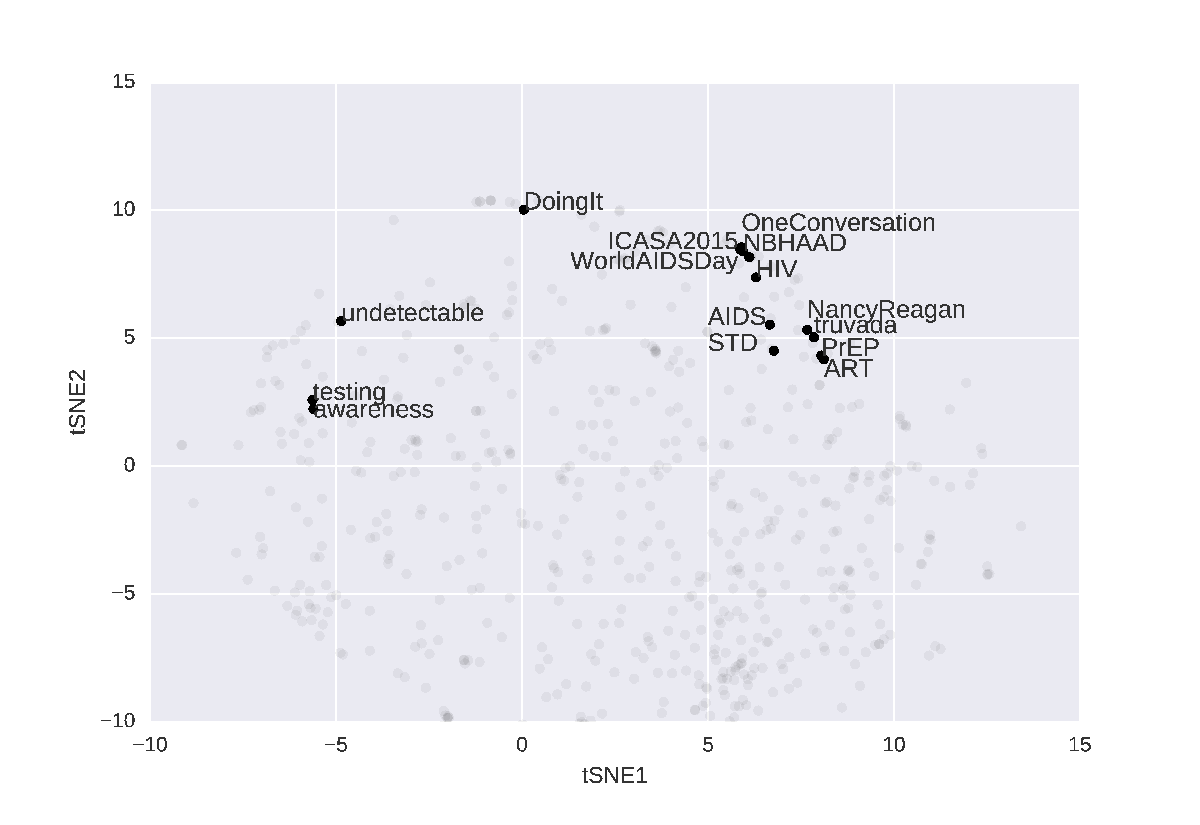
\includegraphics[height=4in, width=6in]{figs/Fig2}
\caption{tSNE plot of relevant word-vectors}
\label{fig:tsne}
\end{figure*}

\subsection{Time Domain}

Next we sought to identify some temporal trends in PrEP related trends. We used Dynamic Topic Modeling (DTM) on our tweet corpus to identify how certain topics change over time. We specified 10 topics and used each week's worth of tweets, over a 30 week period from the 47th week of 2015 to the 14th week of 2016, as our time points.

We identified two topics that showed relevant trends. In topic 5 we see that the keyword `PrEP' increases over time, while `prevention', `drug' and `risk' remain constant (Fig.~\ref{fig:prep}). The term `pill', also from topic 5, declines overtime. These dynamics may indicate that PrEP discussion is becoming more prevalent. This growing trend would be consistent with the fact that while PrEP is still not widely known about among patients and healthcare providers, information about PrEP is slowly entering into national awareness. A study in New York City in 2011 indicated that only 36\% of high risk individuals were aware of PrEP~\cite{mehta2011awareness}.

Other HIV prevention related words such as `pill', `prevention' and `drug' serve as negative controls. They are related to PrEP, but also used in other medical contexts. The fact that they are not increasing, shows us that the increase in PrEP discussion is PrEP-specific.

However, it is hard to tell from these data whether the increased level of PrEP discussion is leading to increased levels of informed patients, medical providers, and adherence. It is possible that stigma, and misinformation is leading to greater levels of PrEP discussion on twitter. We will get more specific, granular understanding of the PrEP discourse in our sentiment analysis section below (see section ``Sentiment Classification'').

% figure 3
\begin{figure}
\centering
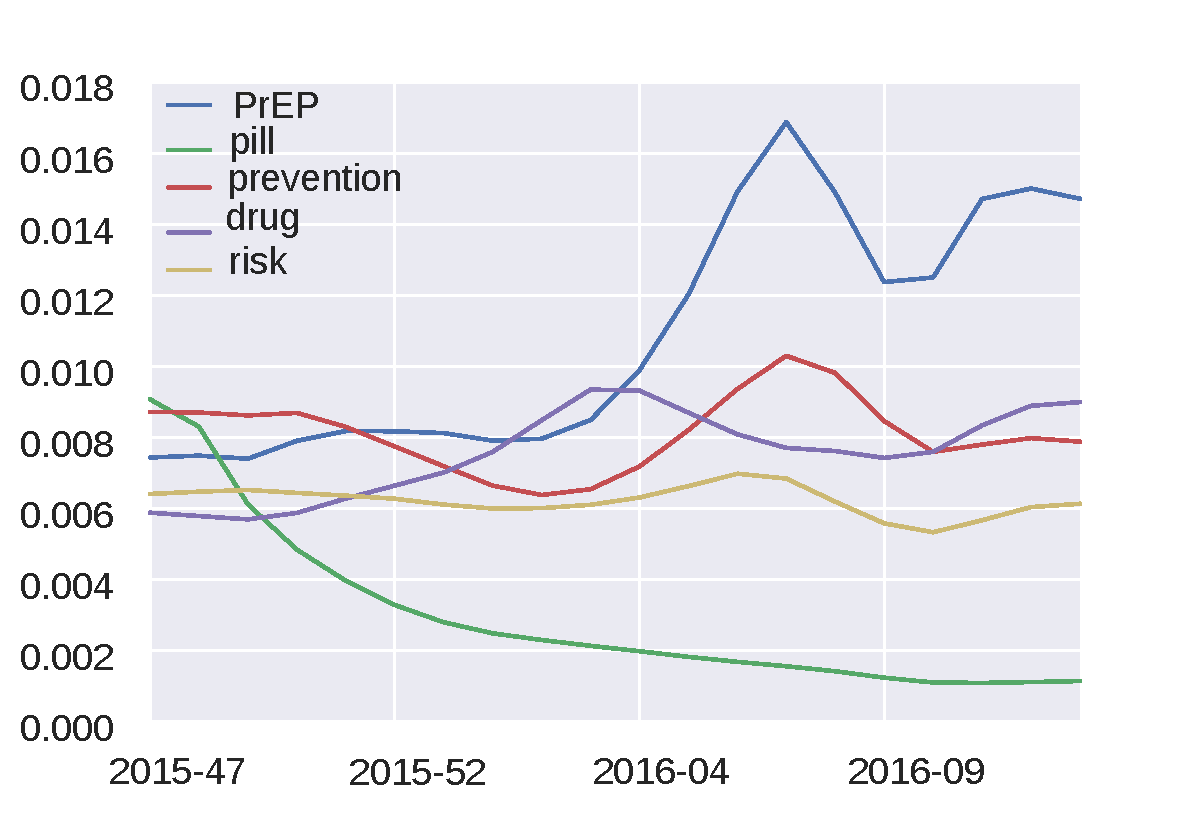
\includegraphics[height=2.5in, width=3.5in]{figs/DTMFig3}
\caption{DTM topic 5 (PrEP related topic) word prevalence over time. Date is YYYY-WW.}
\label{fig:prep}
\end{figure}

We found at least one other DTM topic that showed interesting behavior. We observed that topic 4 captured several keywords related to World AIDS Day (Fig.~\ref{fig:aids}). We can see that ``WorldAIDSDay'', and ``Can'' peak in the 47th week of 2015 and then decline into 2016. This correlates well with the actual date of World AIDS Day, December 1st. Furthermore, while December 1st is World AIDS day, the whole month of December is AIDS Awareness Month. We can clearly see the words `raise' and `awareness' peak later and last longer than the word `WorldAIDSDay' indicating that these words are correlated to the whole month of December. While our PrEP investigation isn't specifically interested in World AIDS Day, or AIDS Awareness Month, this observation serves as a control to validate our ability to accurately identify temporal events using DTM. 

% figure 4
\begin{figure}
\centering
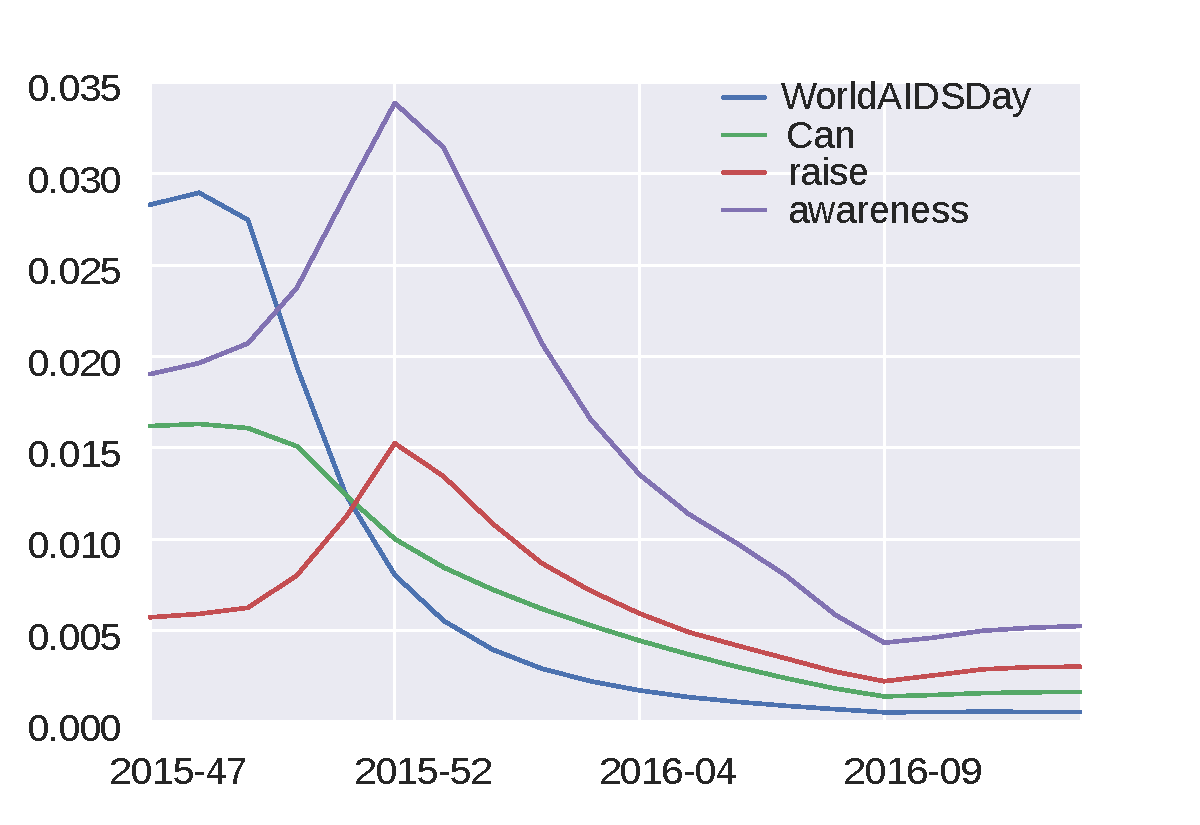
\includegraphics[height=2.5in, width=3.5in]{figs/DTMFig4}
\caption{DTM topic 4 (WorldAIDSDay related topic) word prevalence over time. Date is YYYY-WW.}
\label{fig:aids}
\end{figure}

Together, the DTM results demonstrate our ability to extract relevant HIV and PrEP related information from Twitter that accurately captures time-dependent fluctuations. Public health professionals should be able to monitor these temporal trends to determine the relative interest in PrEP, and other HIV related keywords as they are discussed over time.

\subsection{User Timeline Analysis}

We wanted to identify what Twitter users that mentioned PrEP were discussing in their other tweets. We identified users that were most similar to PrEP using our doc2vec results, then downloaded their recent tweet history, up to their last 3000 tweets. We selected the top 500 users that had at least 200 total words in the combined tweets of their tweet history. For each user, we concatenated their timeline of tweets, and performed LDA topic modeling on the resulting set of user-timeline documents (Fig.~\ref{fig:lda}).

% figure 5
\begin{figure*}
\centering
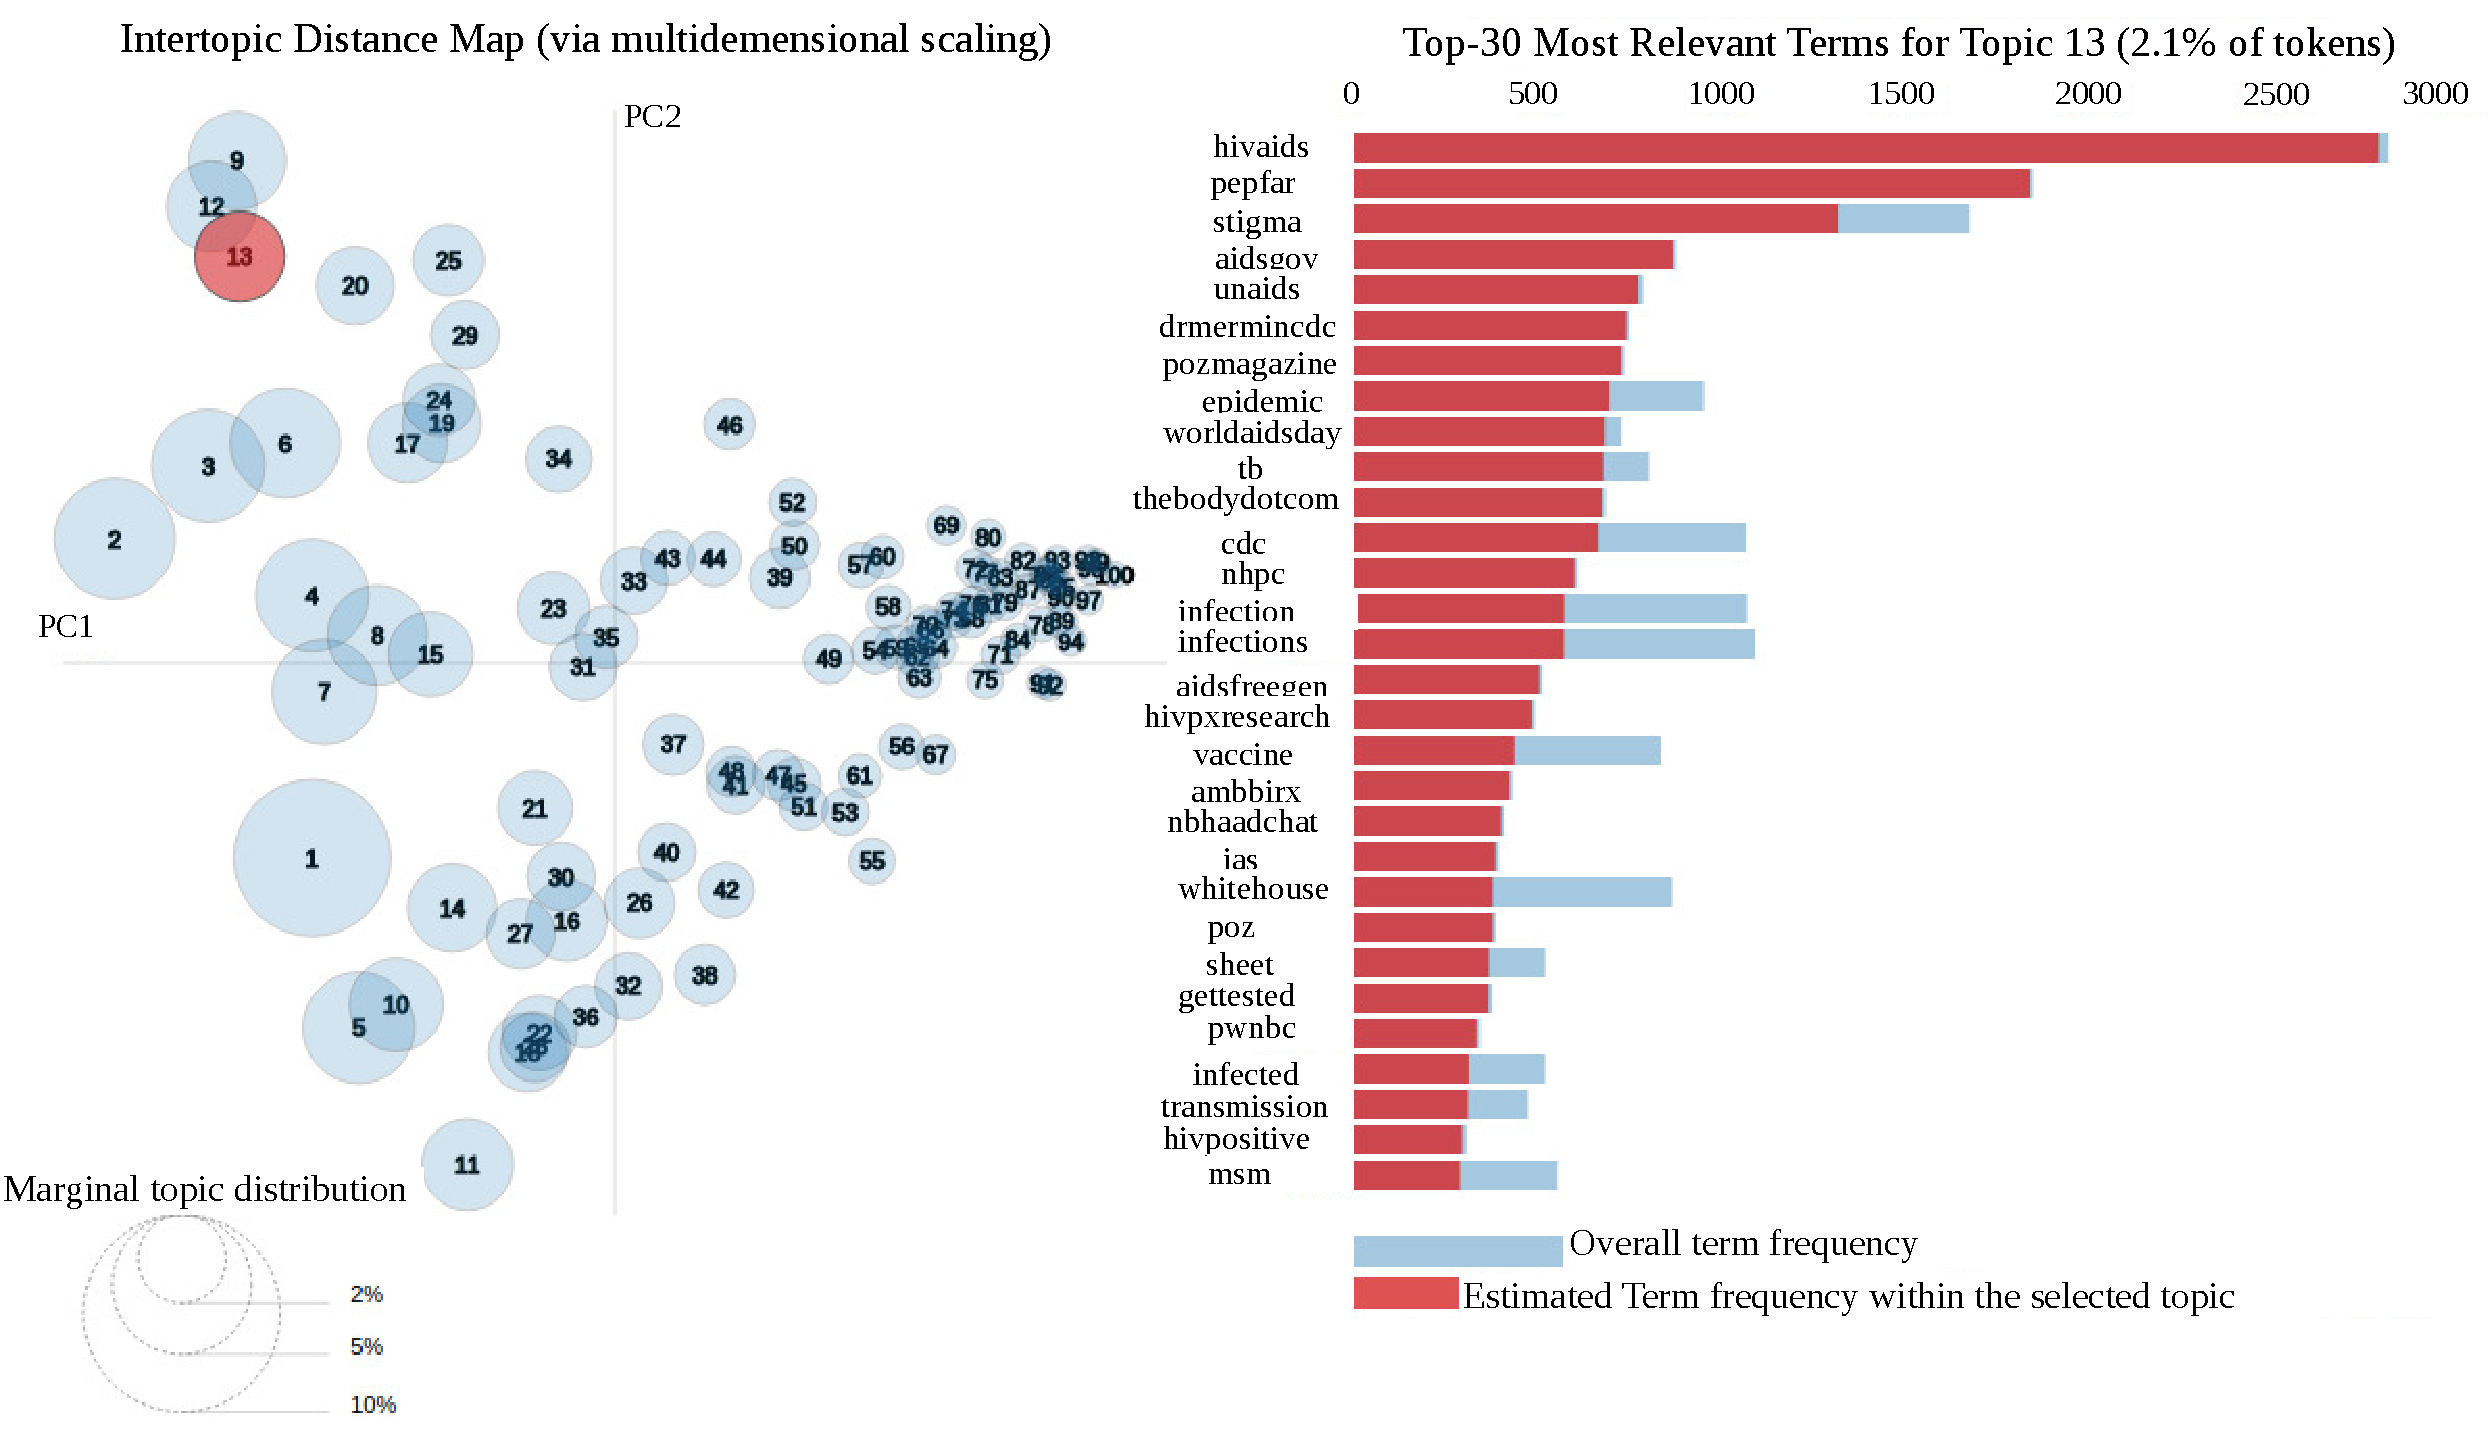
\includegraphics[height=4.5in, width=7.0in]{figs/fixFig5}
\caption{LDA topic modeling for the top 500 users related to PrEP.}
\label{fig:lda}
\end{figure*}

We performed LDA on the users' timelines using the pyLDAvis python package from GraphLab~\cite{low2014graphlab}. We specified 100 topics, and found that only one of them was related to HIV (topic number 13, see Figure 5) representing about 2\% of the marginal topic distribution. Topic 13 contained top terms ``hivaids'', ``pepfar'', ``stigma'' and ``aidsgov''. PEPFAR is a governmental organization, The United States President's Emergency Plan for AIDS Relief, that is focused on combating the spread of AIDS internationally. Interestingly, we don't see PrEP in the top 30 terms in topic 13. This indicates that among twitter users that talk about PrEP, HIV is a small part of their discussion, and PrEP an even smaller part of their discussion.

We investigated some of the other major topics from users' timelines, and found discussions of other STD's (topics 20, 29 and 17) and other health related terms (topics 12, and 25). The other health and STD-related topics clustered closely with topic 13 in Principle Component (PC) space. Some of the STD-related topics included terms related to LGBTQ, including the social networking platform Grindr in topic 17. Other terms related to STD's include prevention terms such as ``CDC'', ``condoms'', and ``gettested''. Topic 19 is nearby these STD-related topics in PC space, and contains terms related to healthcare and political issues such as ``Obamacare'' and ``ACA'' (Affordable Care Act). This connection between HIV, other STD prevention topics, and political discourse may be relevant in PrEP-based HIV prevention efforts, considering there is in some cases no clear precedent for how preventative therapies like PrEP are covered by health insurance~\cite{liu2014early}.

One of the top words from the HIV-related topic, topic 13, was the term ``stigma'', the term ``endstigma'' was also found in topic 17. Previous studies have shown a variety of stigmas associated and HIV have hampered prevention efforts~\cite{liu2014early}. Our observation of stigma related terms corroborates that there is some discussion of stigma in the context of HIV on Twitter. Public health professionals may be able use the prevalence of the term ``endstigma'' as a way to monitor the efficacy of efforts to end HIV related stigmas.

\subsection{Sentiment Classification}

Previously, we used analyses to summarize the whole Twitter corpus to extract high level trends. For our final analysis, we sought to get a deeper understanding of the data at the individual tweet level. Thus we trained a classifier to classify the sentiment of HIV and PrEP related tweets to be either positive or negative. This classifier would allow public health professionals to quickly identify positive and negative PrEP related tweets to guide HIV prevention efforts. We obtained a set of 1.6 million tweets with binary sentiment labels from Sanders Analytics~\cite{sentimentdata}. Then we trained a simple logistic regression classifier on 1.2 million paragraph-vectors from the sentiment dataset. We found that our classifier had an accuracy of 69\% using a portion of the sentiment tweets not used in training, as a validation set.

We chose to use a relatively simple classifier model (logistic regression) and stop training at 20 epochs of stochastic gradient decent over the corpus, because we wanted to prevent the possibility that we overtrained on our training data. This was especially important because our training and testing data, while both sets of tweets, were separate datasets. We used this trained classifier to classify our PrEP related tweets into positive or negative sentiment labels. We identified the most positive, and the most negative tweets, by log probability, on our full dataset, and positive and negative tweets that specifically mention either PrEP or Truvada. We provide the text from the top three positive and negative tweets from each of the three datasets (Table~\ref{tbl:pos}, Table~\ref{tbl:neg}).

% do a top positive tweets table (also with tweet ID)
% table 3
\begin{table*}
\centering
\caption{Positive sentiment tweets.}
\begin{tabular}{|p{2.5cm}|p{12cm}|} \hline
Category & Text\\ \hline
General & ``RT TOPublicHealth The Works provides testing for HIV anonymous \& rapid test available . Call 416-392-0520 for more info''\\ \hline
General & ``RT FCAA ejaforg announced 5.4 million in grants to support orgs addressing \#HIV in new \& innovative ways!''\\ \hline
General & ``RT HillaryClinton A note on the fight against HIV and AIDS and the people who really started the conversation.''\\ \hline

PrEP specific & ``He won't use condoms because intimacy means more than his health. but he's discovered PrEP. thank goodness.''\\ \hline
PrEP specific & ``PrEP Queensland Aids Council, \#HIV Foundation, Queensland.''\\ \hline
PrEP specific & ``RT JDatTheBody At the core of our programs is belief that young ppl can succeed in take PrEP for HIV prevention. \#NHPC2015''\\ \hline

Truvada specific & ``RT CDC\_HIVAIDS Expanding testing, treatment, \& \#PrEP could prevent up to 185k new \#HIV infections''\\ \hline
Truvada specific & ``Another reason 4 \#Ireland \& \#UK 2 immediately approve \#truvada \& \#PrEP 2 stop \#HIV infections . arleavitt AodhanORiordain MerchantsQuayIR''\\ \hline
Truvada specific & ``RT EvanJPeterson For \#worldAIDSday my early \#PrEP arcticle in strangerslog, art by leviathanleague \#hiv \#truvada \#truvadawhore''\\ \hline

\hline\end{tabular}
\label{tbl:pos}
\end{table*}

% do a top negative tweets table (also with tweet ID)
% table 4
\begin{table*}
\centering
\caption{Negative sentiment tweets.}
\begin{tabular}{|p{2.5cm}|p{12cm}|} \hline
Category & Text\\ \hline
General & ``Also, how f***ing vile of Hillary to say. Reagan did f***ing NOTHING during the AIDS epidemic until it was too late. What a stupid old hag.''\\ \hline
General & ``I wonder why he beat her a** when she was tryna leave like she wasn't gone be running back when she found out she had HIV \& nobody want her''\\ \hline
General & ``Aaannd. Hillary Clinton breathes a sigh of relief that Twitter has left its outrage of her AIDS comments behind to tend to Drumpf debacle.''\\ \hline

PrEP specific & ``RT gaston\_croupier \#Truvada patent's not expired yet but it is sold online as a generic drug? There's something rotten in internet \#PrEP h''\\ \hline
PrEP specific & ``Equality\_MI Syph \& Hep C have gone up 550\% in Gay Men bc many feel tht bc they're on PrEP, they don't need condoms. HIV isn't the only STI.''\\ \hline
PrEP specific & ``Xaviom8 in interviews he says he was adherent. strain was highly resistant, and Truvada wouldn't have blocked it anyways. PrEP didn't fail.''\\ \hline

Truvada specific & ``not surprised at all that someone got HIV on truvada. people get pregnant on birth control. tomato-condoms are still important-tomahto''\\ \hline
Truvada specific & ``Now reading that truvada does not protect against certain strains of the HIV virus. Yet people want to take that risk..''\\ \hline
Truvada specific & ``I think I have conjunctivitis unless truvada cured it overnight cuz im not feeling as horrible today as last night''\\ \hline

\hline\end{tabular}
\label{tbl:neg}
\end{table*}

While the sentiment classification doesn't have perfect sentiment accuracy, we can see in general that the positive tweets are disseminating information about the efficacy and benefits of PrEP related preventions (Table~\ref{tbl:pos}). The positive tweets indicate that PrEP public health informational efforts have had some effect disseminating useful PrEP information on Twitter. 

The negative tweets may be more important than the positive tweets to guide future public health policy corrections. The negative tweets contain concerns that Truvada may not block HIV transmission in all cases (Table~\ref{tbl:neg}). There also seems to be concern that use of Truvada may increase the transmission of non-HIV STDs such as Hepatitis C because some PrEP users stop using condoms. This may indicate that public health professionals need to stress that PrEP users should continue to wear condoms for full protection against other diseases when disseminating PrEP-related health information.

Another negative tweet questions whether Truvada is available as a generic drug. PrEP is currently only available through Gilead's Truvada, though a generic may be available as soon as 2017~\cite{truvadagenericblog}. Current patients must deal with uncertain drug prices, which vary from \$14,000 to \$70~\cite{truvadagenericblog}, and have in some cases, uncertain medical insurance reimbursement status. This tweet highlights both the difficulty of acquiring affordable PrEP medication, and also a level of conflicting information circulating on social media.

Finally we see some contention over national political leadership in the effort to prevent HIV. While political discussions can often get heated, especially on Twitter, the contention can harm concerted efforts to provide consistent governmental leadership in HIV prevention. Public health officials may consider stressing that unity in health policy at the federal level is important to protect the population from the spread of HIV.

The last tweet in the positive tweets (Table~\ref{tbl:pos}), referencing the hashtag ``\#truvadawhore'', links to a blog article written by Evan Peterson titled ``The Case for PrEP, or How I Learned to Stop Worrying and Love HIV-Positive Guys''~\cite{caseforprep}. Evan is an HIV-negative individual who adheres to a daily PrEP regimen to protect himself from HIV. Evan finds that for himself, the side effects and inconveniences associated with taking daily Truvada are worth the protection, noting that he also practices safe sex, and gets tested regularly. Evan addresses the hashtag \#truvadawhore, which originated with a Huffington Post article titled ``Truvada Whores?''~\cite{truvadawhore} which expressed concern toward the increased sexual risk taking of some Truvada patients. Evan provides a rebuttal, noting that many HIV-negative individuals on Truvada, including himself and people he knows, are responsible and cautious about the risks they are taking. He explains that taking daily Truvada may actually be an indication that individuals are more educated and responsible with respect to their sexual health. Further large scale quantitative measurements, including large scale medical surveys, will be needed to determine whether or not taking Truvada correlates positively or negatively with risk-taking behaviors.

\section{Conclusions}

In this article we use a variety of NLP techniques to analyze a tweet corpus in order to monitor the national social media discussion for HIV prevention. We identified several notable trends. We found that PrEP discussion activity is increasing on Twitter, and also that people who mention PrEP also talk about general health, STDs, stigma, and politics.

By picking out the tweets most relevant to PrEP, and classifying these tweets as positive or negative, we quickly identified core concepts important to the online PrEP discussion. We identified two important arguments for and against PrEP. Blogger Steven Banning hypothesizes that PrEP adoption could lead to unintended consequences and unhealthy risk seeking behavior. The contrary hypothesis, described by blogger Evan Peterson, suggests that PrEP adherence is a product of healthy, responsible, at-risk individuals who are gaining an effective form of HIV protection. These opposing arguments were identified automatically using large scale data mining of social media. Further investigation and data analyses of social media data together with other health data may be able to quantify PrEP and Truvada's effectiveness in the ongoing effort to prevent HIV infection, as well as highlight possible strategies to maximize PrEP effectiveness.

Future analyses may also take further advantage of the rich Twitter API. Rather than passively collecting data, intelligent chatbots could be deployed to interact with HIV and PrEP-tweeters. This would enable researchers to conduct large scale social-media-based health surveys and directly observe the dynamics of the discussion.

% conference papers do not normally have an appendix


% use section* for acknowledgment
\section*{Acknowledgments}

The authors would like to thank our collaborators in the Georgia HIV research community, including individuals at The University of Georgia, The Center for Disease control, Oak Ridge National Laboratory, Emory University, The Georgia Department of Public Health and the Kaiser Family Foundation.



% trigger a \newpage just before the given reference
% number - used to balance the columns on the last page
% adjust value as needed - may need to be readjusted if
% the document is modified later
%\IEEEtriggeratref{8}
% The "triggered" command can be changed if desired:
%\IEEEtriggercmd{\enlargethispage{-5in}}

% references section

% can use a bibliography generated by BibTeX as a .bbl file
% BibTeX documentation can be easily obtained at:
% http://mirror.ctan.org/biblio/bibtex/contrib/doc/
% The IEEEtran BibTeX style support page is at:
% http://www.michaelshell.org/tex/ieeetran/bibtex/
\bibliographystyle{IEEEtran}
% argument is your BibTeX string definitions and bibliography database(s)
\bibliography{draft}
%
% <OR> manually copy in the resultant .bbl file
% set second argument of \begin to the number of references
% (used to reserve space for the reference number labels box)
%\begin{thebibliography}{1}
%
%\bibitem{IEEEhowto:kopka}
%H.~Kopka and P.~W. Daly, \emph{A Guide to \LaTeX}, 3rd~ed.\hskip 1em plus
%  0.5em minus 0.4em\relax Harlow, England: Addison-Wesley, 1999.
%
%\end{thebibliography}




% that's all folks
\end{document}


